
\chapter{The "XYZ" Prototype System}

% NOTES / TODOs:
%
% Architecture scheme, implementation
% callback functions, hot plugin
% js-select selectors
% List of condition operators
% Why JS, why wasnt it used before? is it used now?
% Transactions in businesses, find use case. how would we lose events?
% Terminierungsproblem (compiler bau), loesungsansaetze



\section{Event Triggers}

Event Gathering is the E in ECA and without one of these letters such a system would not run.
It is of utmost importance to find as much as possible ways to get data into a system.



\subsection{Polling for Events}



\subsection{Webhooks}
Which 



\section{Actions}



\section{ECA Rules}



\section{Architecture}



\section{Asynchronous Systems \& Closures}
% NOTES / TODOs:
%
% Variable bindings
% Closures (https://developer.mozilla.org/en-US/docs/Web/JavaScript/Guide/Closures)$
% Closures are functions that refer to independent (free) variables. 
% In other words, the function defined in the closure 'remembers' the environment in which it was created in.

% write about arallel as well?

Certain optimization approaches and programming language concepts require special attention to avoid common pitfalls.
If such approaches and concepts come together, which is the case when closures are used in asynchronous systems, random inconsistencies will be the result if they are not taken care of.


Looking at an example of sequential code execution ( Figure~\ref{fig:Closures_Synchronous} ), we see that function execution of fA is halted until function fB is finished.
If fB happens to be a latency-driven I/O operation the completion of fA could be deferred for a relatively long time.
While the application waits for the completion of the I/O operation, some remaining operations in fA could eventually already be executed without causing any race conditions.

\begin{figure}[h!]
\centering
  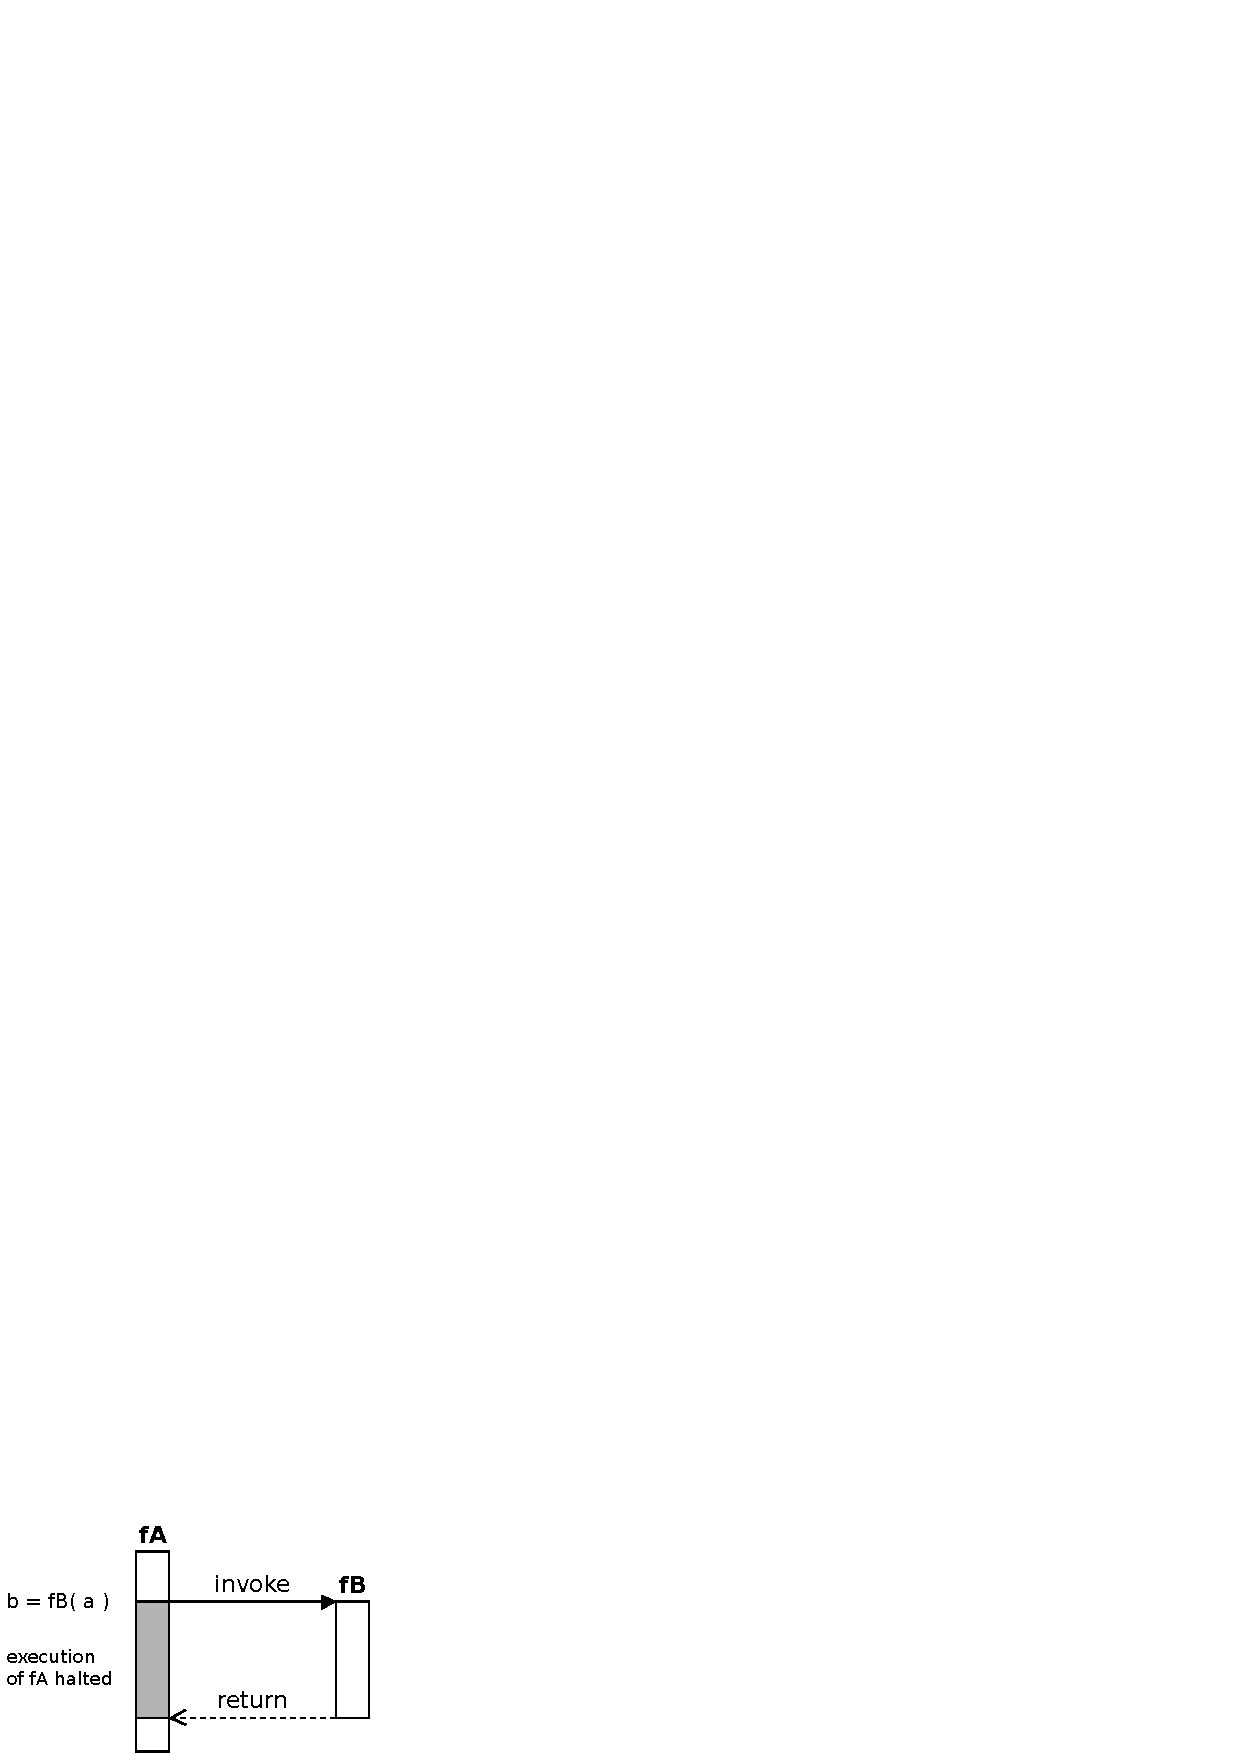
\includegraphics{figures/Closures_Synchronous}
\caption{Synchronous Function Calls}
\label{fig:Closures_Synchronous}
\end{figure}

Non-blocking operations are a remedy for optimzed resource allocation and opens ways to overcome such unnecessary resource bindings.
Asynchronous code execution allows non-blocking and thus scalable applications.
Processing any kind of latency-driven I/O operation asynchronously ( e.g. filesystem access and socket communication ) exploits resources that would otherwise be bound while waiting for completion.
Such operations are processed and completed whenever required resources are available.
Often other operations depend on the completion of asynchronous operations, hence their execution needs to be deferred.
This required code execution deferral is achieved through the application of callback functions.
Any code placed in a callback function, which is assigned to an asynchronous operation, is only executed when the respective asynchronous operation completed.
This leads to stacking of functions and operations



Such callback functions are passed as arguments to asynchronous operations and executed as soon as the operation finishes.

By deferring the executiong of operations that depend on the 

asynchronously results in dynamic code which exploits .

together with closures they 

Test reference Figure ~\ref{fig:Closures_Synchronous}



\begin{figure*}[htb]
%\begin{center}
\centering
%,angle=-90
  \makebox[\textwidth][c]{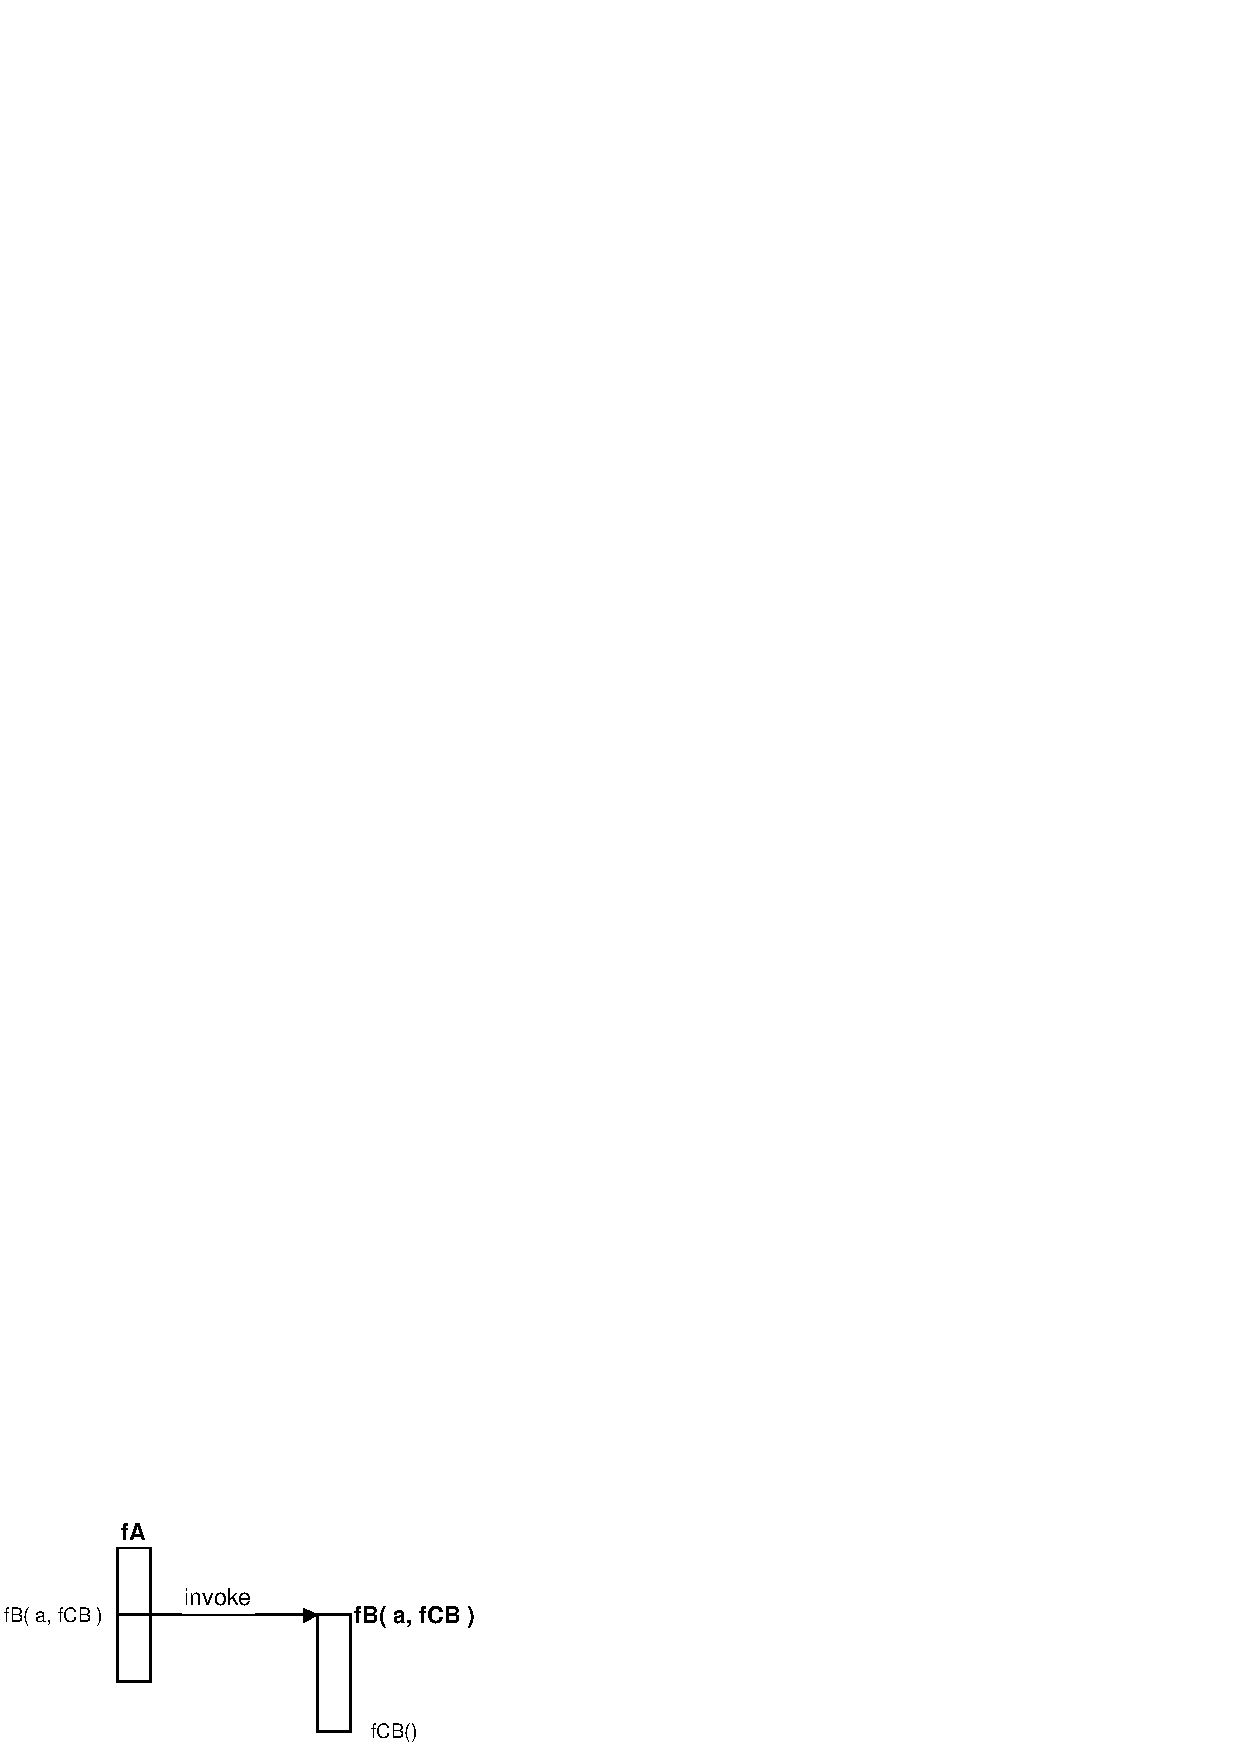
\includegraphics{figures/Closures_Asynchronous}}%
\caption{Asynchronous Function Calls}
%\end{center}
\end{figure*}


\begin{figure*}[htb]
%\begin{center}
\centering
%,angle=-90
  \makebox[\textwidth][c]{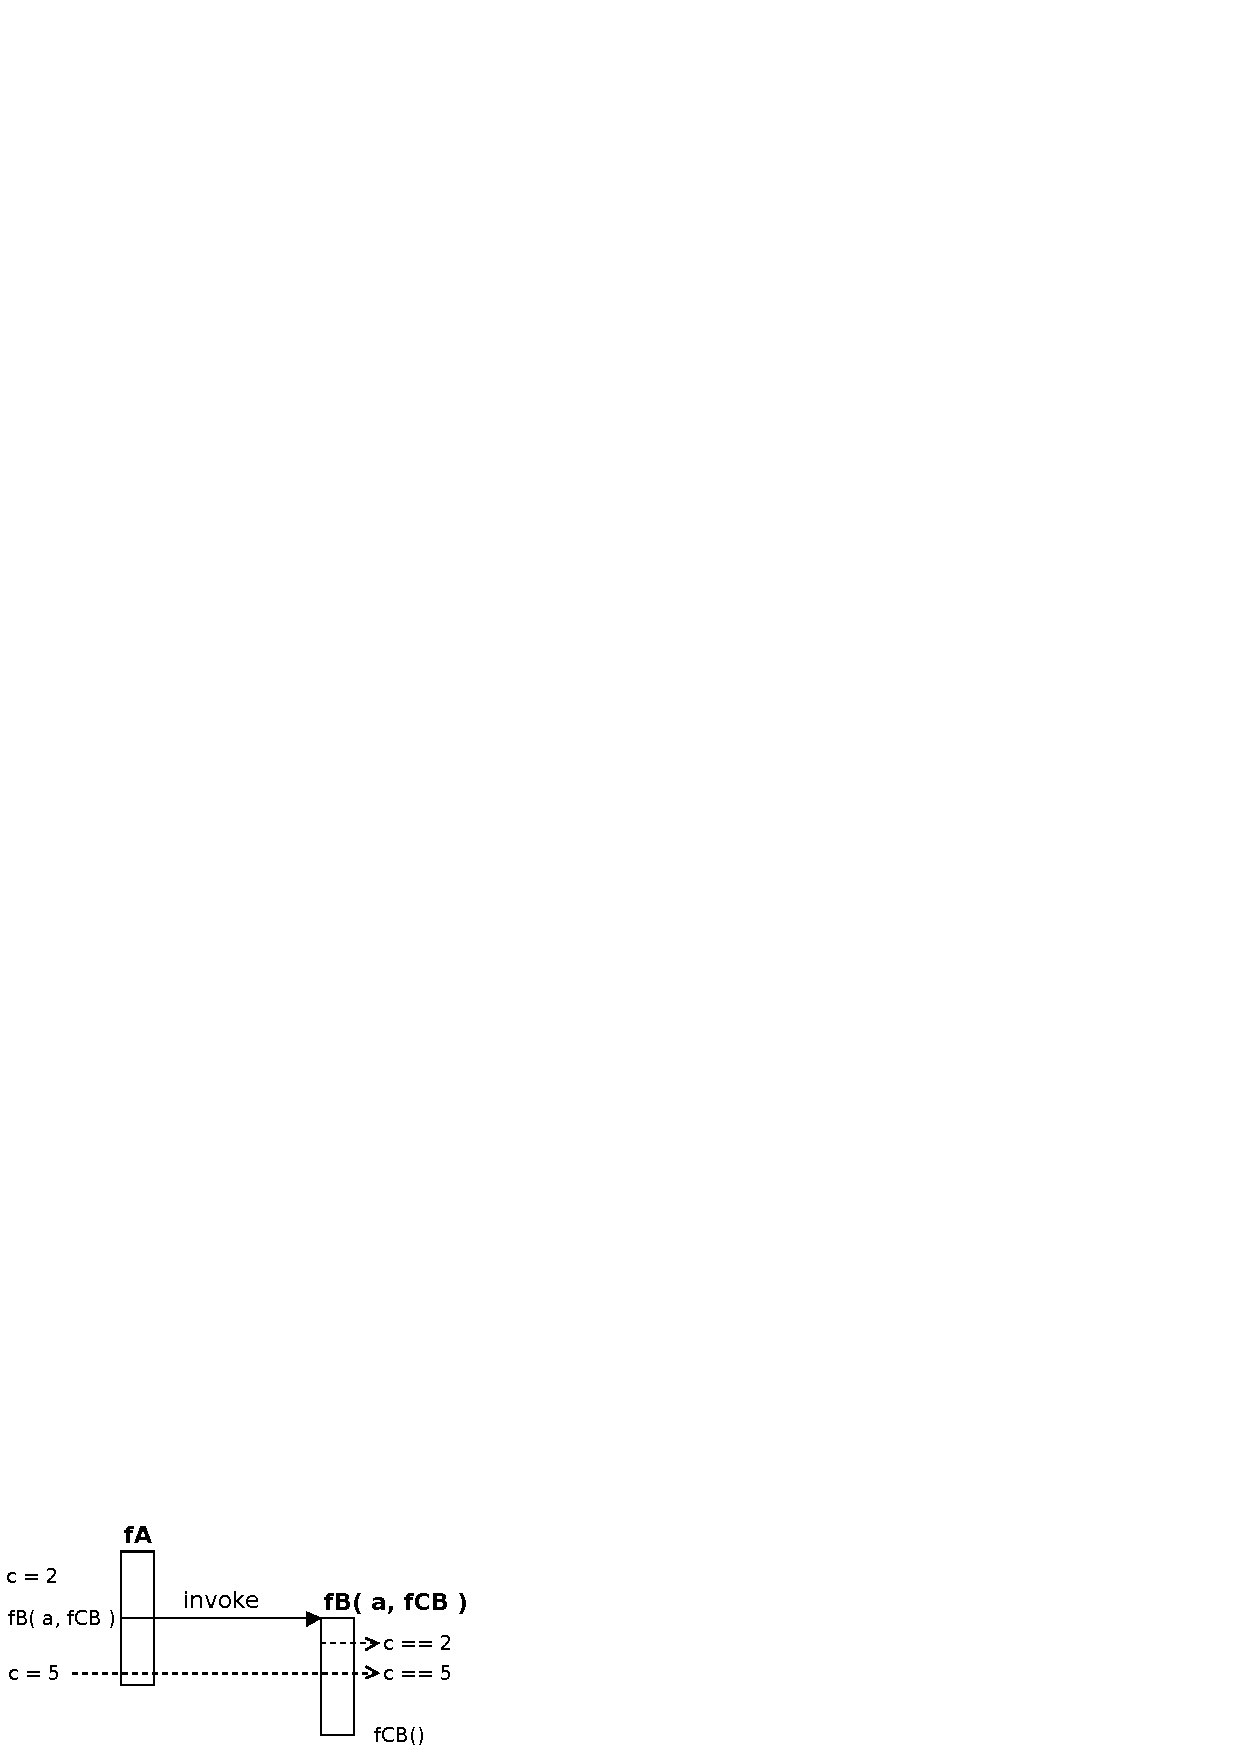
\includegraphics{figures/Closures_Closure-1}}%
\caption{Closure Scope}
%\end{center}
\end{figure*}


\begin{figure*}[htb]
%\begin{center}
\centering
%,angle=-90
  \makebox[\textwidth][c]{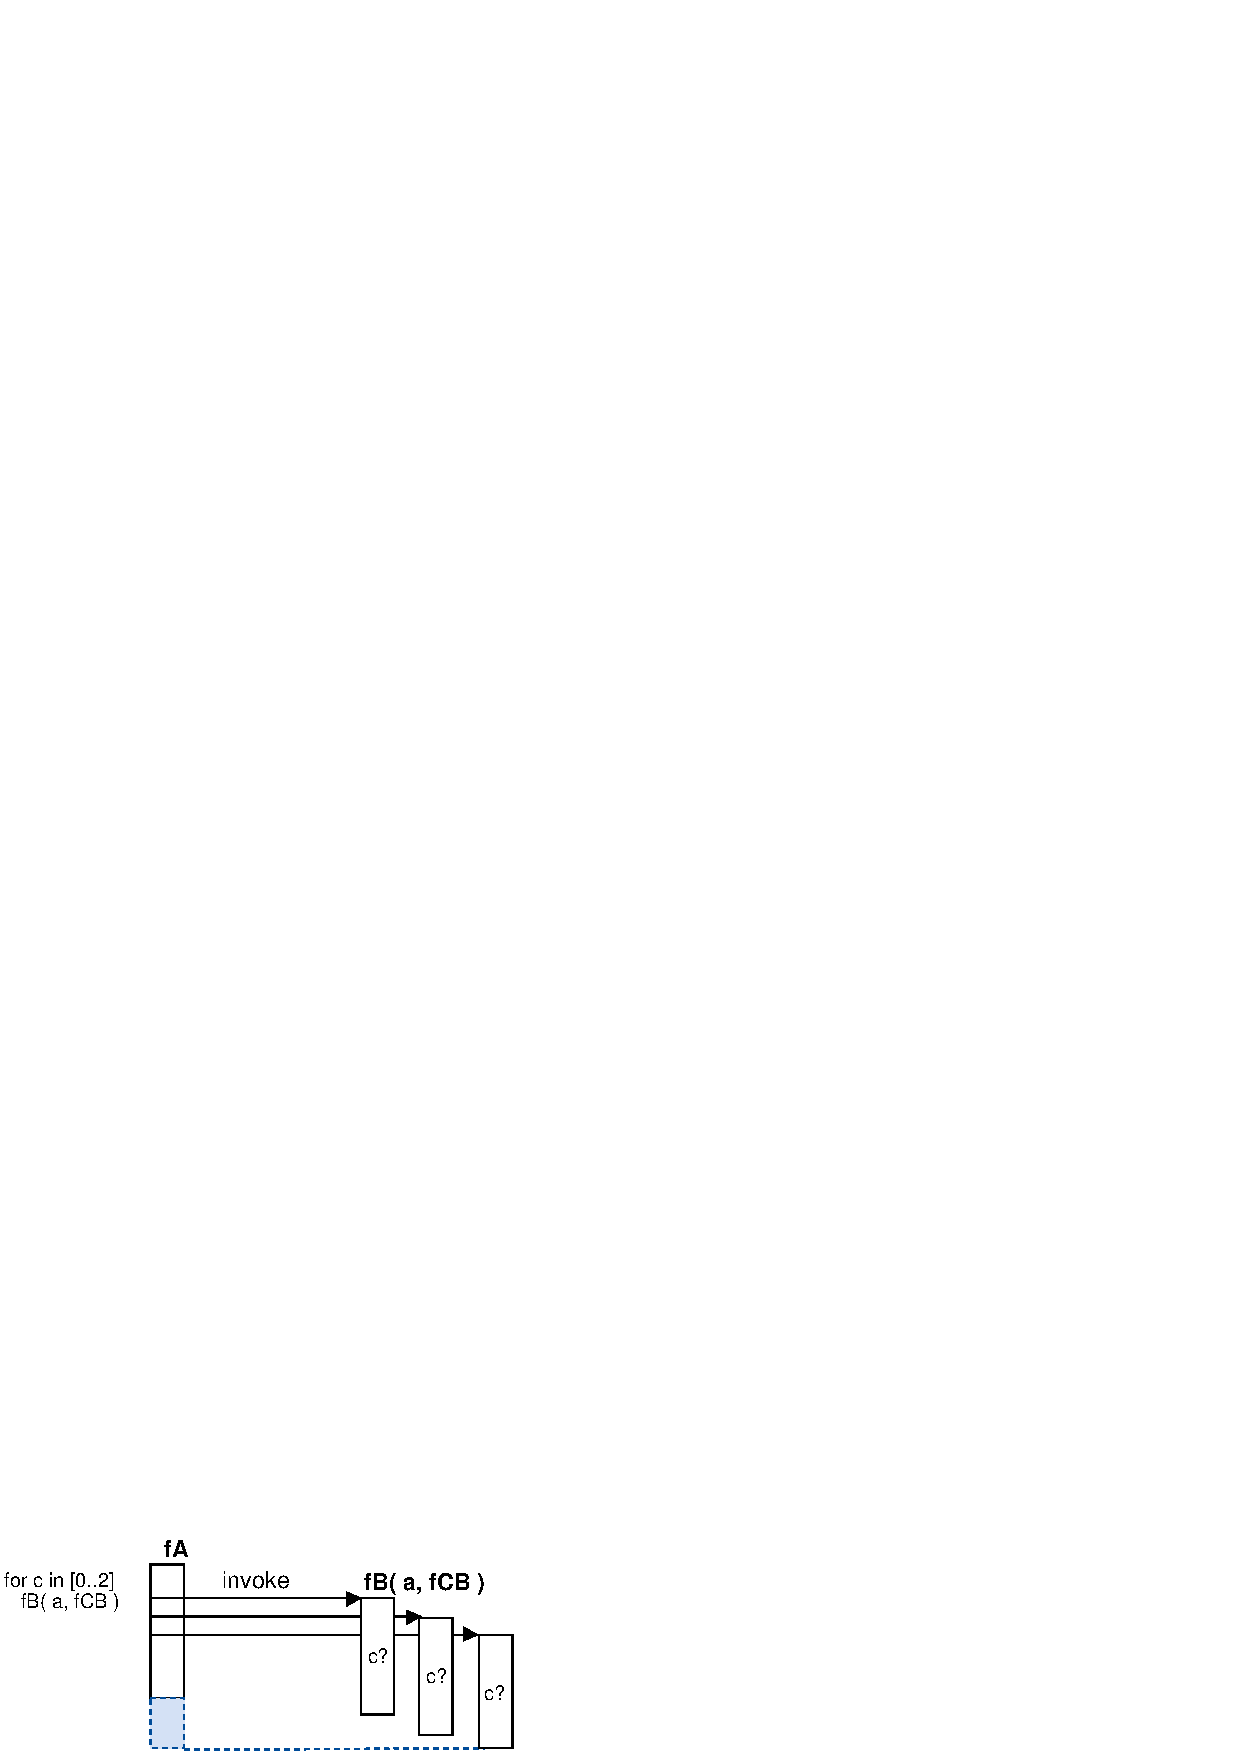
\includegraphics{figures/Closures_Closure-2}}%
\caption{Closure Scope}
%\end{center}
\end{figure*}


\begin{figure*}[htb]
%\begin{center}
\centering
%,angle=-90
  \makebox[\textwidth][c]{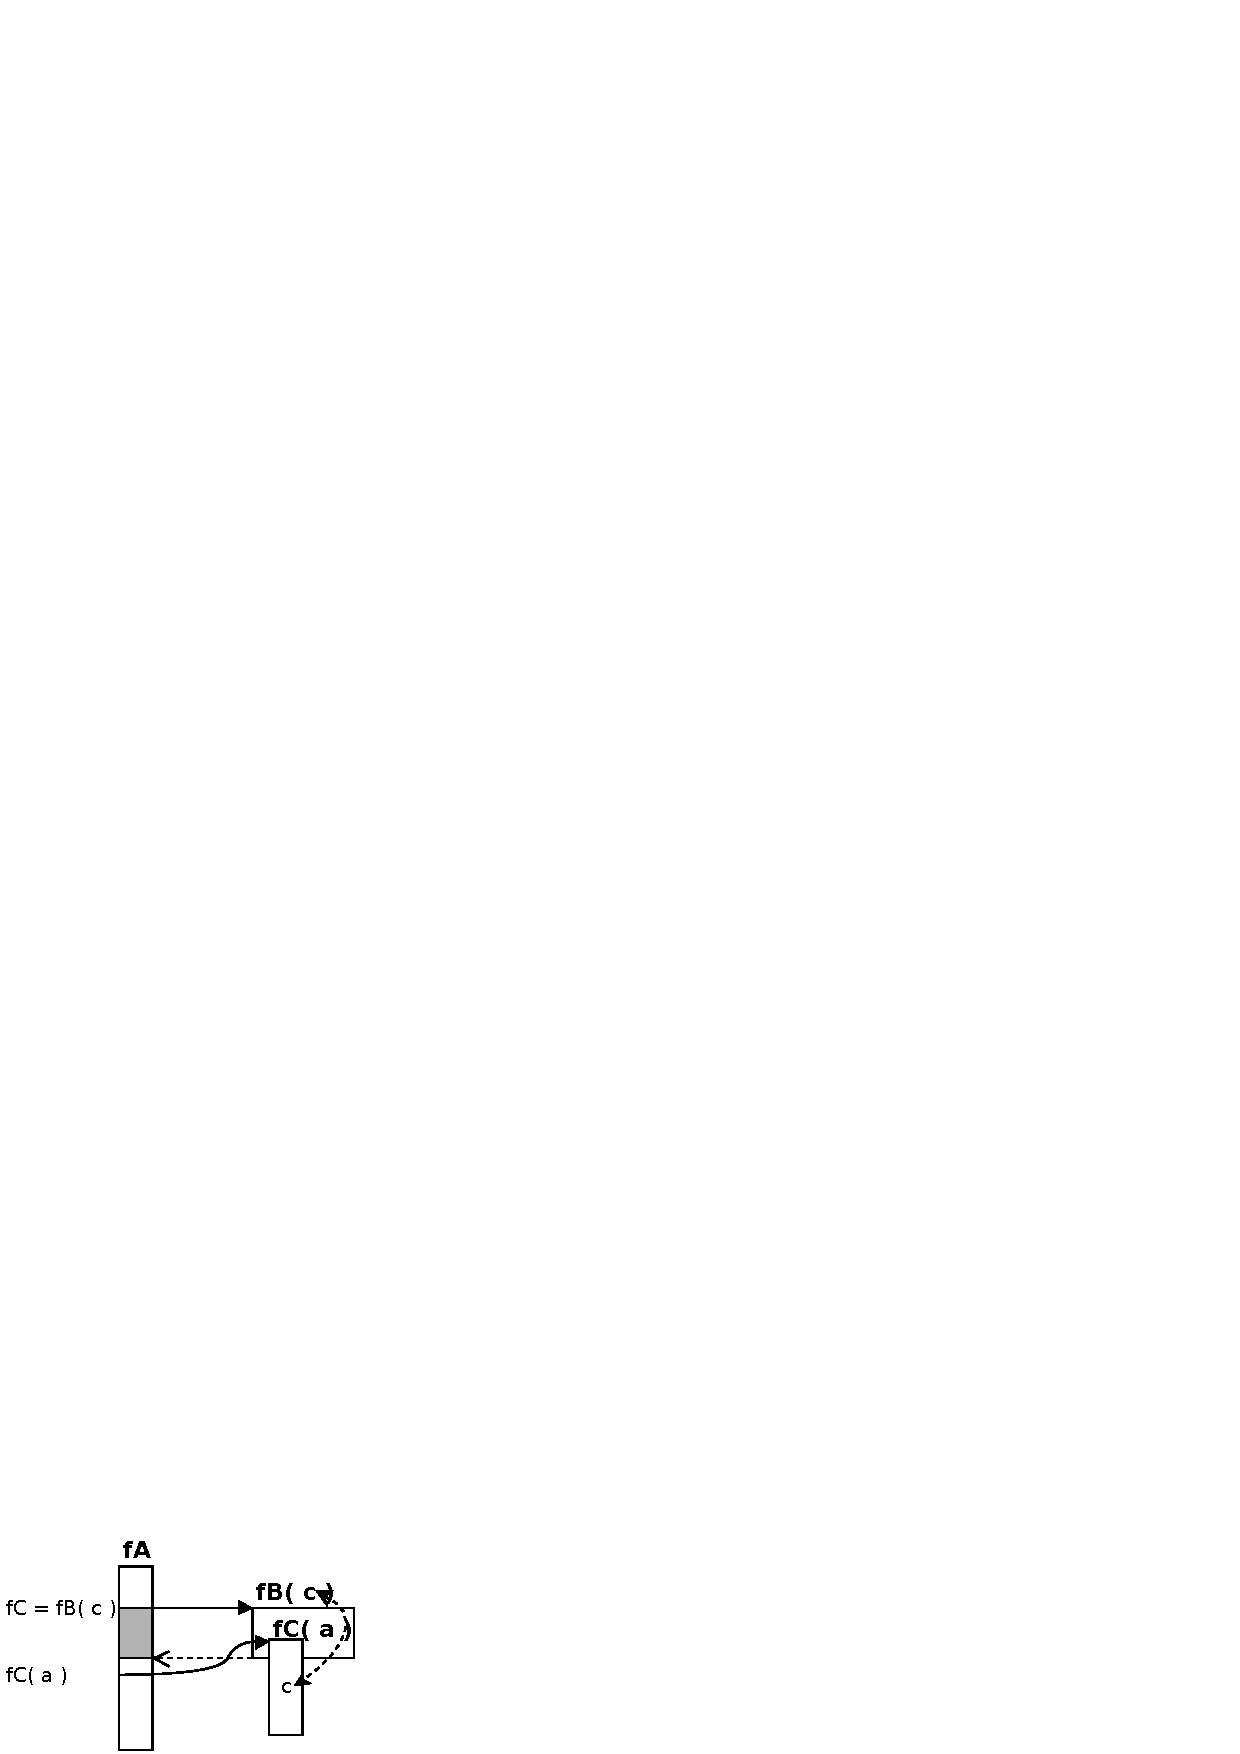
\includegraphics{figures/Closures_Closure-3}}%
\caption{Closure Scope}
%\end{center}
\end{figure*}

% Error tracing
% Apply variable number of function arguments to function
